\documentclass[
  journal=pasa,
  manuscript=review, %% or "review"
  year=2021,
  volume=37,
]{cup-journal}

\usepackage{microtype,siunitx,booktabs}
\usepackage{natbib}
\usepackage{tabularx}
\usepackage{enumitem,bbding}
\usepackage{longtable}
\sisetup{detect-all,separate-uncertainty=true}

%------------------VISITADOR-------------------------------------------------

\title{Aplicación de la metodología KDD en el diagnostico de la morbilidad por cáncer de mama en la ciudad de Pereira-Risaralda}

\author{Jorge Armando Millán Gómez}
\affiliation{Minería de Datos, Universidad Distrital "Francisco José de Caldas", Facultad de Ingeniería, Bogotá, Colombia}
\email[J. A. Millán]{jamillang@correo.udistrital.edu.co}

%\author{M. Sokolowski}
%\affiliation{International Centre for Radio Astronomy Research, Curtin University, Bentley, WA6102, Australia}
% \alsoaffiliation{Joint first authors}

%\author{R. Wayth}
%\affiliation{International Centre for Radio Astronomy Research, Curtin University, Bentley, WA6102, Australia}

%\author{D. Ung}
%\affiliation{International Centre for Radio Astronomy Research, Curtin University, Bentley, WA6102, Australia}

%\handlingeditor{Excellent E Editor}

\doi{10.1017/pasa.2022.32}

\received {20 03 2022}
\revised  {20 03 2022}
\accepted {20 03 2022}
\published{19 Abril 2022}

\keywords{minería de datos, KDD, cáncer de mama, pronostico, Colombia.}
 %% First letter not capped
% \jel{Q11; Q12; D81; M31}
% \msc{Q14; Q18; E21}
% \abbreviations{
%     BDHS: Bangladesh Demographic and Health Survey, 
%     IDA: Fe-deficiency anaemia, 
%     IFA: Fe-folic acid, 
%     MNP: multiple micronutrient powder, 
%     VAD: vitamin A deficiency
% }
\begin{document}

\chapter{Metodología DSM-BCD}

Dado los problemas presentados de los proyectos basados en datos, y el estudio de diversas metodologías propuestas por varios autores, se propone la metodología \textit{DSM-BCD (Data Science Methodology for Breast Cancer Diagnosis)}. En la figura \ref{DSM-BCD} se puede visualizar las fases de la metodología DSM-BCD.

\begin{figure*}[!htb]
	\centering
	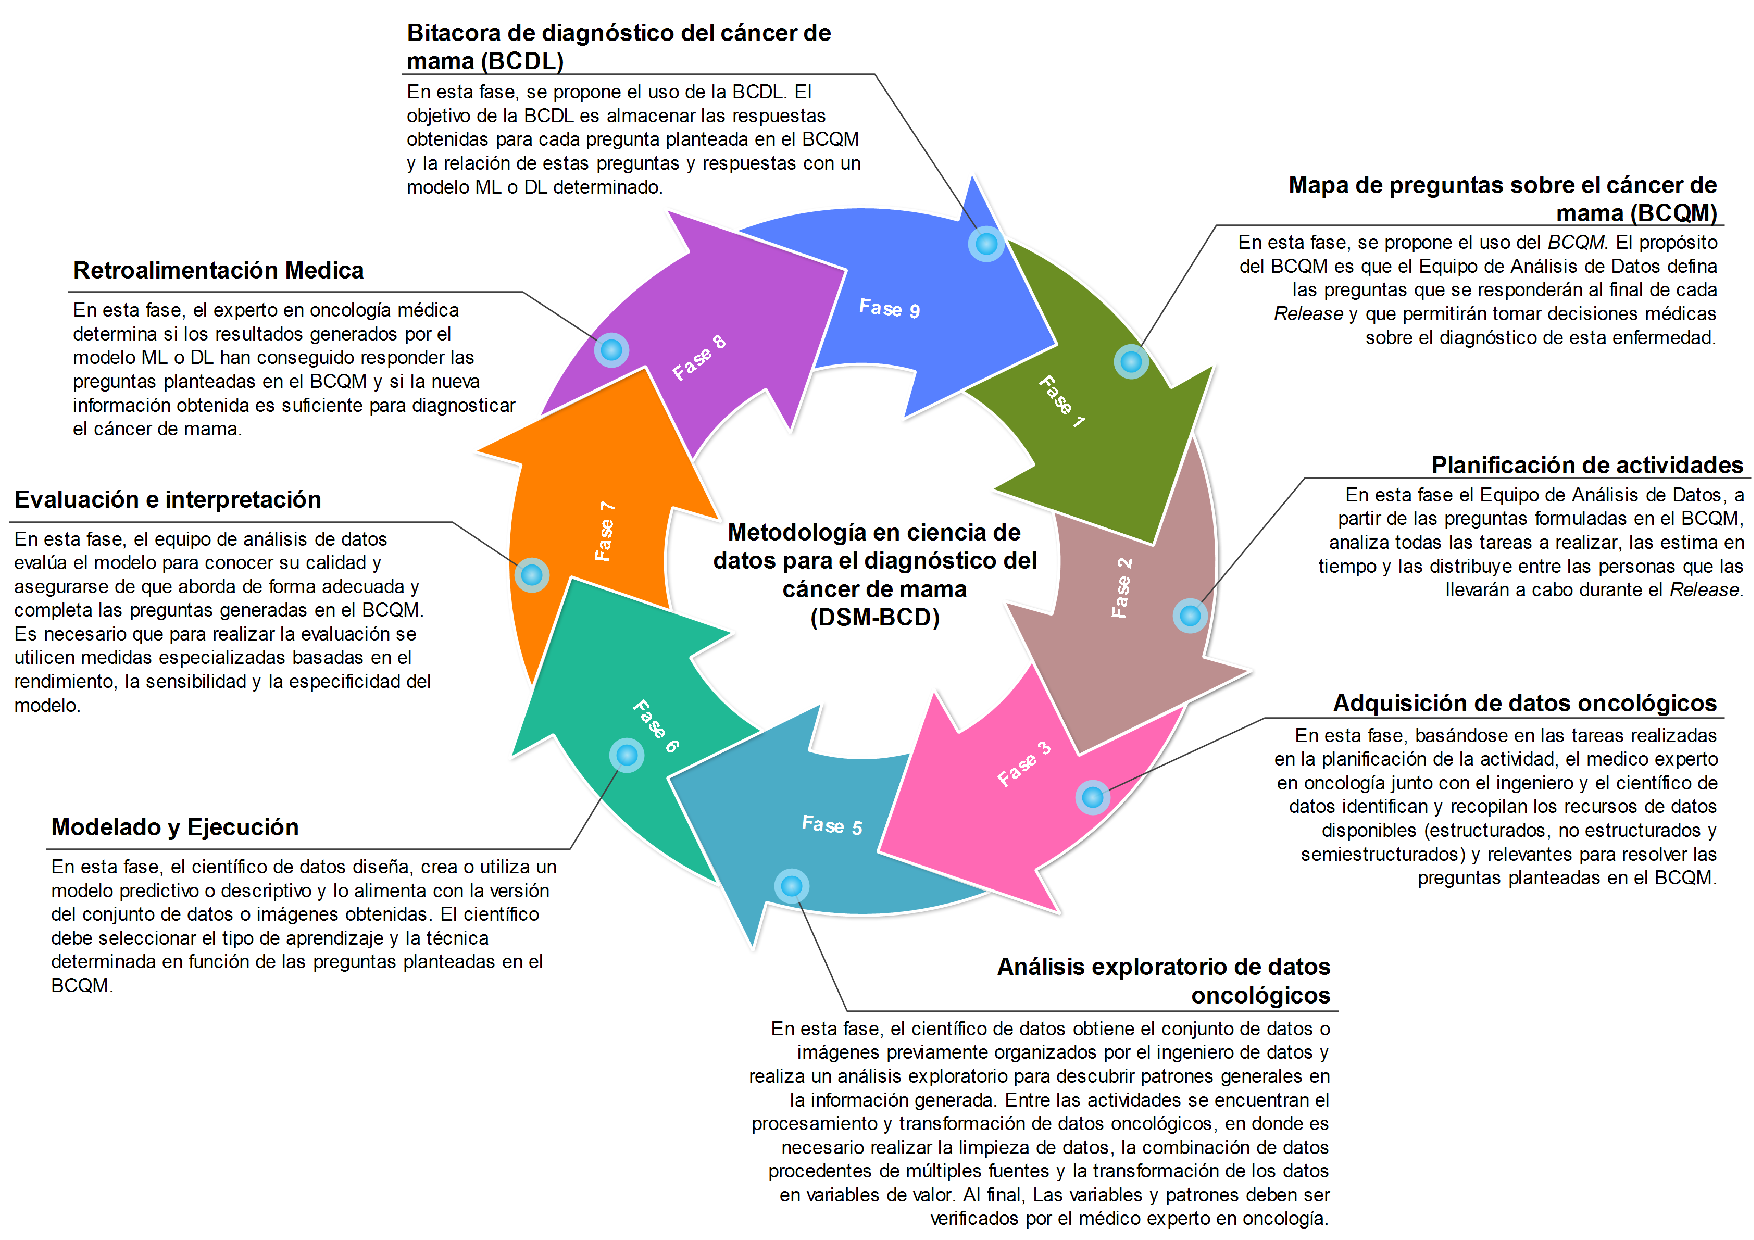
\includegraphics[width=0.9
	\linewidth]{IMAGENES/DSM-BCD_SPANISH.pdf}
	\caption{Metodología en ciencia de datos para el diagnóstico del cáncer de mama 
		(DSM-BCD)}
	\label{DSM-BCD}
\end{figure*}

Esta metodología tiene como base el \textit{manifestó ágil} aplicado a un contexto de resultados basados en datos. Dado lo anterior \textit{DSM-BCD} no se enfoca en evaluar la precisión de las técnicas de ML y DL sino su objetivo principal es generar valor a los datos en el tiempo mas corto posible para que los médicos diagnostiquen de manera ágil el cáncer de mama. Para lograrlo \textit{DSM-BCD} integra la perspicacia medica y los resultados obtenidos por las técnicas de ML y DL en una retroalimentación continua generada en cada \textit{Release} para producir mayor eficacia en la toma de decisiones

 En \textit{DSM-BCD}, se propone la conformación de un \textit{Data Analysis Team}. Este equipo debe estar encabezado por el medico experto en oncología, al menos un ingeniero de datos y un científico de datos. Se recomienda que el equipo este conformado por un máximo de 5 personas para facilitar el trabajo en equipo y la comunicación interna.
 
 Para comprender mejor el uso de DSM-BCD, se realizó un análisis descriptivo basados en datos genéticos característicos de tumores generados por los tipos de cáncer \textit{Carcinoma ductal invasivo (IDC)} y \textit{Carcinoma lobulillar invasivo (LBC)}, en donde se logró determinar que el IDC y LBC son enfermedades molecularmente distintas con rasgos genéticos característicos, lo que proporciona información importante para la estratificación de los pacientes permitiendo realizar diagnostico clínico ágil con precedentes para un tratamiento puntual.


\section{Fase 1: Mapa de preguntas sobre el cáncer de mama (BCQM)} 
En esta fase se propone el uso de un mapa de preguntas sobre el cáncer de mama (BCQM). El proposito del \textit{BCQM} es que el \textit{Data Analysis Team} defina las preguntas que serán resueltas al finalizar cada \textit{Release} y que permitirán tomar decisiones medicas con respecto al diagnostico de esta enfermedad. En la figura \ref{BCQM} se observa la estructura del BCQM.

\begin{figure}
	\centering
	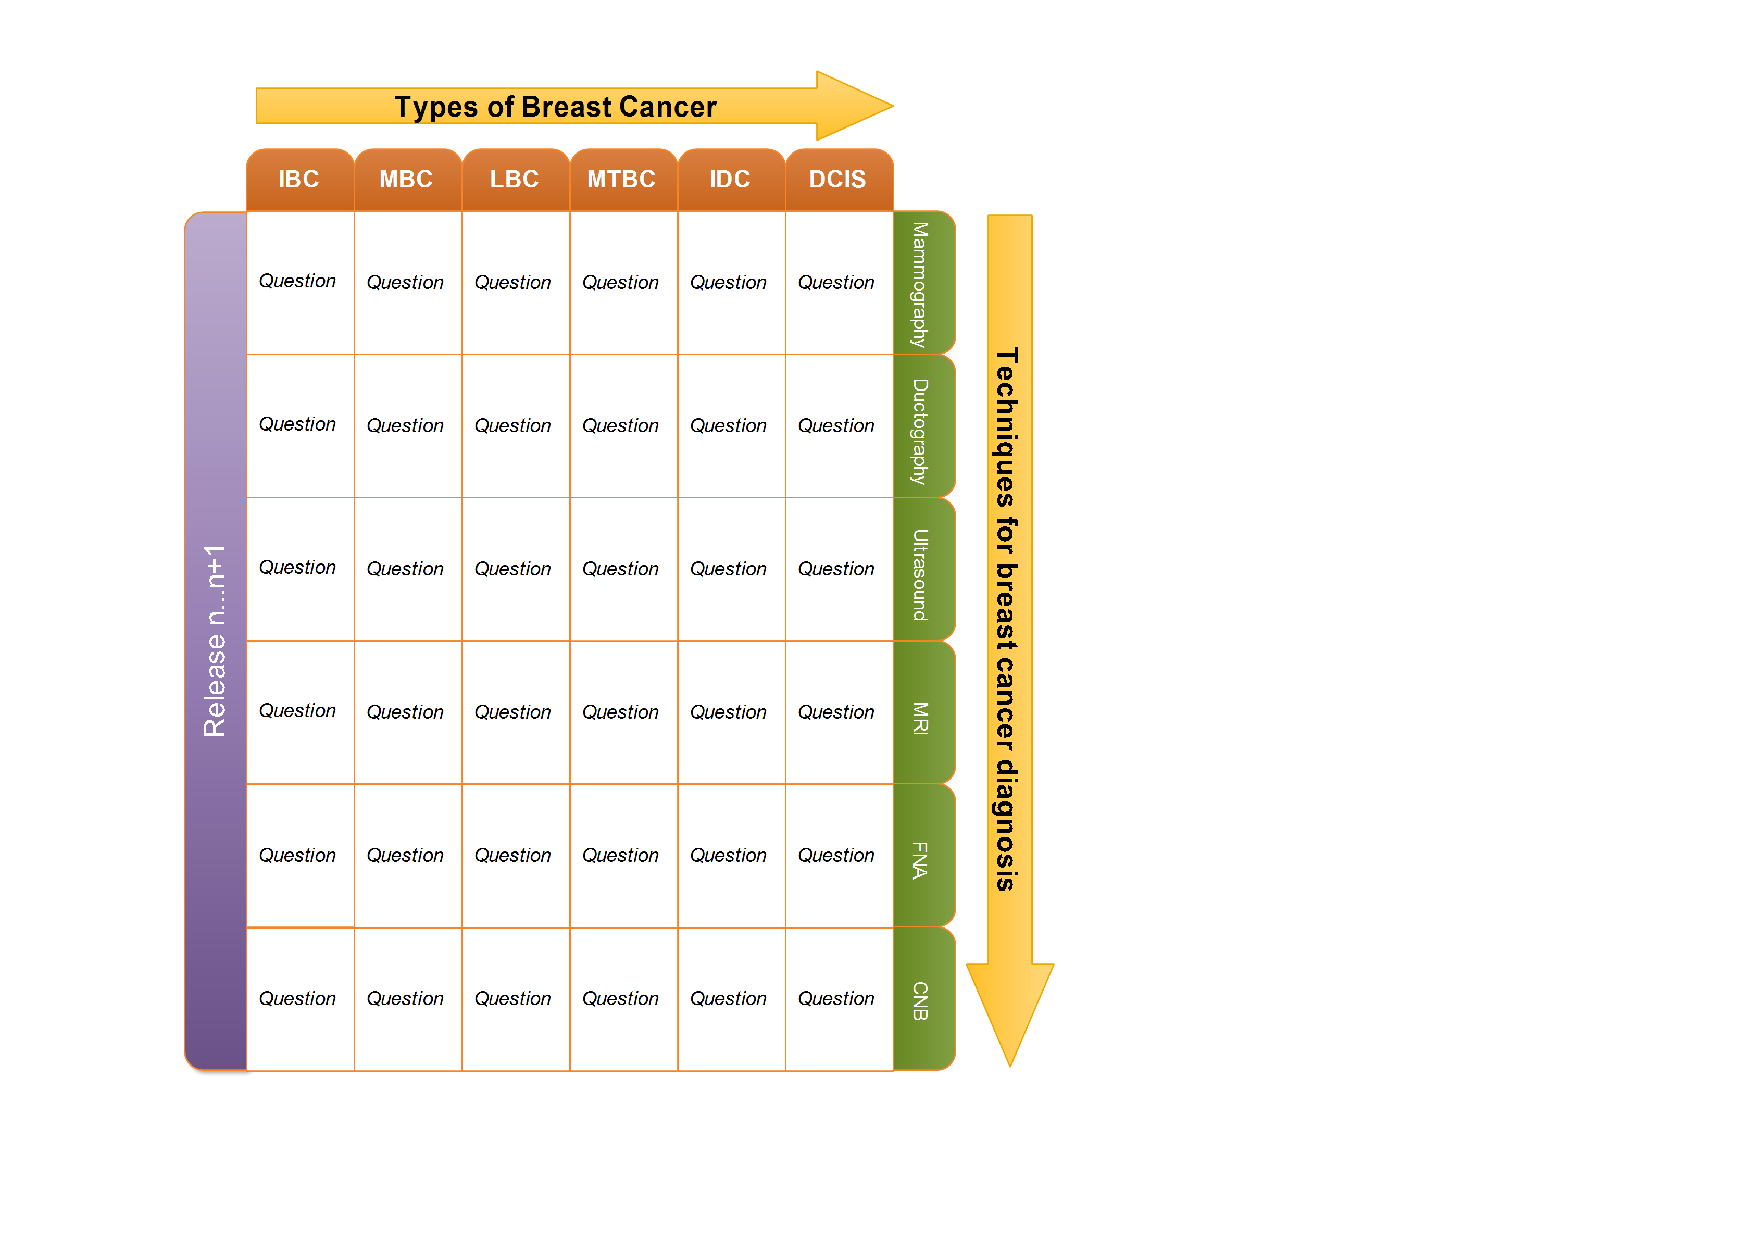
\includegraphics[width=0.6
	\linewidth]{IMAGENES/BCQM}
	\caption{Mapa de preguntas basados en los tipos de cáncer de mama \textit{inflamatorio (IBC)}, \textit{mucinoso (MBC)}, \textit{Lobulillar (LBC)}, \textit{Tumores mixtos (MTBC)}, \textit{Carcinoma ductal invasivo (IDC)} y \textit{Carcinoma ductal in situ (DCIS)}}
	\label{BCQM}
\end{figure}

El BCQM permite plantear preguntas relacionadas a los tipos de cáncer de mama y a las técnicas para el diagnostico de la misma. De modo que al finalizar el tiempo de cada \textit{Release}, el cual puede variar entre 1 y 4 semanas, las preguntas serán respondidas según el análisis de datos generado, y el medico podrá tomar una decisión de valor. Cabe resaltar, que es posible tener una o mas preguntas relacionadas a una técnica y a un tipo de cáncer de mama por cada \textit{Release}, razón por la cual es posible encontrar correlaciones entre las variables características de cada tipo de cáncer encontrando así patrones ocultos en los diferentes conjuntos de datos. Adicionalmente, el BCQM permite identificar a que técnica para el diagnostico de cáncer mama esta relacionada la pregunta a resolver, lo cual de antemano hace posible conocer el tipo información (imágenes o datos) y el algoritmo  ML o DL requerido para dar solución al problema. Así mismo, el BCQM permite definir desde la fase inicial el tipo de modelo predictivo o descriptivo según el enfoque analítico generado por la pregunta planteada. Sintetizando, el uso de BCQM facilita la comprensión del problema medico y permite identificar previamente la técnica, el tipo de información y enfoque que debe ser utilizado para el análisis de datos.  

\section{Fase 2: Planeación de actividades}
En esta fase el \textit{Data Analysis Team} basado en las preguntas realizadas en el BCQM analiza todas las tareas que hay que llevar a cabo, las estiman en tiempo y las distribuyen entre las personas que las van a realizar durante el \textit{Release}. Dado que el BCQM nos permite conocer de antemano el tipo de cáncer de mama y la técnica para el diagnostico de esta enfermedad, el científico de datos con ayuda del medico puede definir el origen de datos, lo cual va a permitir conocer el tipo, cantidad y peso de la información. Dado lo anterior, es recomendable que el equipo tenga al menos un ingeniero datos, ya que el es el encargado de tomar los datos y convertirlos en información significativa para que el científico pueda realizar el respectivo análisis.   

\section{Fase 3: Adquisición de datos oncológicos}
En esta fase, con base a la tareas realizadas en la planeación de actividades, el medico experto en oncología junto con el ingeniero y el científico de datos identifican y reúnen los recursos de datos disponibles (estructurados, no estructurados y semiestructurados) y relevantes para solucionar las preguntas planteadas en el \textit{BCQM}. Cabe resaltar, que en la metodología \textit{\textit{DSM-BCD}} es factible tener varios conjuntos de datos o imágenes que están relacionados a un tipo de cáncer de mama y una técnica de diagnostico, por lo tanto  el \textit{Data Analysis Team} puede tener a varios científicos respondiendo preguntas diferentes en un mismo \textit{Release}. Como consecuencia, al final se pueden obtener como resultado múltiples respuestas y una posible correlación entre las diversas variables oncológicas.  Asimismo, en esta fase el \textit{Data Analysis Team} debe definir la infraestructura de datos necesaria según la cantidad de información a procesar, lo cual permitirá proyectar la escalabilidad, alcance y distribución de dicha información. 

Para este caso de estudio, se utilizaron variables genéticas características de marcadores tumorales  basados en los siguientes tipos de cáncer de mama:

\begin{itemize}
	\item \textit{Carcinoma ductal invasivo (IDC)}:  Este tipo de cáncer ocurre cuando las células anormales de la mama se diseminan por todos los tejidos mamarios.
	
	\item \textit{Carcinoma lobulillar invasivo (LBC)}: Este tipo de cáncer ocurre cuando las células anormales de la mama se diseminan en lóbulo mamario.
\end{itemize}

Estas variables fueron obtenidas del conjunto de datos denominado \textit{“Breast Invasive Carcinoma (TCGA, Cell 2015)”} creado a partir del proyecto de carcinoma invasivo de mama \textit{Comprehensive Molecular Portraits of InvasiveLobular Breast Cancer} \cite{Ciriello2015} basado en el \textit {Atlas del Genoma del Cáncer (TCGA\footnote{Acrónimo de “The Cancer Genome Atlas (TCGA)”, en inglés })} cuya finalidad es catalogar cambios moleculares de importancia biológica responsables de la aparición de cáncer haciendo uso de la secuenciación genómica y la bioinformática \cite{TCGA2023}. Los datos fueron descargados del sitio público \textit{cBioPortal} para la genómica del cáncer  (\url{https://www.cbioportal.org/study/summary?id=brca_tcga_pub2015}). Cabe resaltar, que el conjunto de datos contiene un total de 817 muestras de tumores de mama que  se perfilaron con 6 plataformas moleculares: Análisis del número de copias somáticas basado en array, Secuenciación del exoma completo, perfil de metilación del ADN basado en array, secuenciación del ARN mensajero, secuenciación de microARN (miARN) y array de proteínas en fase inversa (RPPA), como se ha descrito previamente en \cite{Bass2014}. Un comité de patología revisó y clasificó todos los tumores en 490 IDC, 127 LBC, 88 casos con características mixtas de IDC e LBC, y 112 con otras histologías.

Este conjunto de datos consta de un tamaño de $818$ filas y $110$ columnas. Las variables se describen en la tabla \ref{brca_tcga_pub2015_clinical_data}: 

\begin{table*} [!htb]
	\footnotesize
	\begin{threeparttable}
		\caption{Conjunto de datos del Carcinoma invasivo de mama (TCGA, Cell 2015).}
		\label{brca_tcga_pub2015_clinical_data}
		\begin{tabular}{p{1cm} p{4cm} p{10cm}} \toprule	
			\begin{center}$N$\end{center}   
			&\begin{center}Variable\end{center}             
			&\begin{center}Descripción\end{center}      
			\\ \hline	
			%-----------------------------------------------------------------------------------
			1
			&Study ID
			&Código de identificación del estudio.
			\\ \hline
			%-----------------------------------------------------------------------------------
			2
			&Patient ID
			&Código de identificación del paciente.
			\\ \hline
			%-----------------------------------------------------------------------------------
			3
			&Sample ID
			&Código de identificación de la muestra.
			\\ \hline
			%-----------------------------------------------------------------------------------
			4
			&Diagnosis Age
			&Edad a la que se diagnosticó por primera vez una afección o enfermedad.
			\\ \hline
			%-----------------------------------------------------------------------------------
			5
			&American Joint Committee on Cancer Metastasis Stage Code
			&Código para representar la ausencia o presencia definida de diseminación a distancia o metástasis (M) a localizaciones a través de canales vasculares o linfáticos más allá de los ganglios linfáticos regionales, utilizando los criterios establecidos por el Comité Conjunto Americano del Cáncer (AJCC).
			\\ \hline
			%-----------------------------------------------------------------------------------
			6
			&Neoplasm Disease Lymph Node Stage American Joint Committee on Cancer Code
			&Los códigos que representan el estadio del cáncer en función de los ganglios presentes (estadio N) según criterios basados en múltiples ediciones del Manual de Estadificación del Cáncer de la AJCC.
			\\ \hline
			%-----------------------------------------------------------------------------------
			7
			&Neoplasm Disease Stage American Joint Committee on Cancer Code
			&La extensión de un cáncer, especialmente si la enfermedad se ha propagado desde el lugar original a otras partes del cuerpo según los criterios de estadificación de la AJCC.
			\\ \hline
			%-----------------------------------------------------------------------------------
			8
			&American Joint Committee on Cancer Publication Version Type
			&Versión o edición del American Joint Committee on Cancer Cancer Staging Handbooks, publicación del grupo formado con el propósito de desarrollar un sistema de estadificación clínica del cáncer que sea aceptable para la profesión médica estadounidense y compatible con otras clasificaciones aceptadas.
			\\ \hline
			%-----------------------------------------------------------------------------------
			9
			&American Joint Committee on Cancer Tumor Stage Code
			&Código de T patológico (tumor primario) para definir el tamaño o la extensión contigua del tumor primario (T), utilizando los criterios de estadificación del AJCC.
			\\ \hline
			%-----------------------------------------------------------------------------------
			10
			&Brachytherapy first reference point administered total dose
			&Primer punto de referencia dosis total administrada en la Braquiterapia .
			\\ \hline
		\end{tabular}
	\end{threeparttable}
\end{table*}

\section{Fase 4: Análisis Exploratorio de datos oncológicos}

En esta fase, el científico obtiene el conjunto de datos o imágenes que fueron organizados previamente por el ingeniero y realiza un \textit{Análisis exploratorio de datos} para descubrir patrones generales en la información generada. Cabe resaltar, que en esta fase el acompañamiento del medico experto en oncología es de vital importancia, ya que los datos o imágenes que van ser explorados por el científico pueden contener variables que pueden tener o no un valor significativo para el experto, ayudando así a determinar si el análisis planteado para responder la pregunta va o no por un buen camino, de modo que es posible que se agreguen o eliminen diversas variables para lograr el resultado esperado. Adicionalmente, es necesario que los diversos análisis generados estén apoyados con gráficas que sean entendibles por todo el \textit{Data Analysis Team}, esto con el proposito de aportar ideas, y desde esta fase ir encontrando posibles correlaciones entre las variables oncológicas.

\section{Fase 5: Procesamiento y transformación de datos oncológicos}
En esta fase, se abarcan todas las actividades para construir el conjunto de datos o imágenes que se utilizará en la siguiente etapa de modelado y ejecución. Entre las actividades del procesamiento y transformación de datos oncológicos, están la limpieza de datos, combinar datos de múltiples fuentes y transformar los datos en variables de valor. En esta fase, es importante el trabajo en equipo y la comunicación continua entre el ingeniero y el científico de datos para tratar los valores no válidos o faltantes, eliminar duplicados, dar un formato adecuado y combinar archivos, tablas y plataformas. Adicionalmente, el medico experto en oncología deberá proporcionar un visto bueno para proceder con la siguiente fase. Esto dado que al ser experto en el tema de dominio tiene un conocimiento mas profundo de las variables o imágenes que esta observando, y si existiese información innecesaria para el diagnostico del cáncer de mama es posible depurar dicha información para que no afecte el entrenamiento y posterior ejecución del modelo de ML y DL.

\section{Fase 6: Modelado y Ejecución}
En esta fase, el científico de datos diseña, crea o utiliza un modelo predictivo o descriptivo y lo alimenta con la versión del conjunto de datos o imágenes obtenidos en la fase de procesamiento y transformación. En esta fase, el científico debe seleccionar el tipo de aprendizaje (supervisado, no supervisado y por refuerzo) y la técnica determinada (regresión, clasificación, clustering, CNN, RNN, etc.) acorde a las preguntas planteadas en el \textit{BCQM}. Hay que mencionar que en esta fase el \textit{Data Analysis Team} debe definir junto al medico experto en oncología la tolerancia de error permitida en el modelo, esto dado a que la sensibilidad de los análisis puede variar dependiendo del tipo de cáncer de mama y la técnica de diagnostico. Es probable que el científico de datos pruebe múltiples algoritmos con sus respectivos parámetros para encontrar el mejor modelo para las variables oncológicas disponibles. Cabe resaltar, que es de vital importancia que los modelos propuestos no tengan problemas de sobre-ajuste o infra-ajuste ya que esto puede generar resultados erróneos o poco significativos. Adicionalmente, el científico de datos en cuestión junto al \textit{Data Analysis Team} deben definir la infraestructura a nivel de servidor necesaria para el entrenamiento y prueba del modelo según la cantidad de información a procesar, esto con el proposito de generar resultados acertados en el menor tiempo posible en pro de cumplir las tareas definidas en la fase de planeación de actividades y dar valor a los datos oncológicos una vez finalice el \textit{Release}.

\section{Fase 7: Evaluación e Interpretación}
En esta fase, el \textit{Data Analysis Team} evalúa el modelo para comprender su calidad y garantizar que este aborda las preguntas generadas en el \textit{BCQM} de manera adecuada y completa. Es necesario que para realizar la evaluación se utilicen medidas especializadas basadas en el rendimiento, sensibilidad y especificidad del modelo. Adicionalmente, los resultados obtenidos deben ser entendibles por el medico experto en oncología, en donde se garantice que dichos resultados sean interpretados correctamente y estén relacionados a la estadificación y los biomarcadores del cáncer de mama. Es importante que el medico junto al científico de datos ajusten el modelo según las necesidades. Dado que se esta trabajando con datos médicos sensibles, es necesario que al modelo final se aplique a un conjunto de validación para realizar una evaluación final. Además, el \textit{Data Analysis Team} puede asignar al modelo pruebas de \textit{significancia estadística} como prueba adicional para comprobar la respuesta obtenida a la pregunta generada. Esta prueba adicional es fundamental para justificar la implementación del modelo. Finalmente, dado que en el \textit{BCQM} se pueden plantear múltiples preguntas relacionadas a diferentes tipo de cáncer de mama y técnicas de diagnostico durante el \textit{Release}, es necesario que los científicos con ayuda del ingeniero de datos unan, si es posible, los resultados obtenidos en una matriz o mapa de calor para identificar el coeficiente de correlación entre dos o mas variables oncológicas. Esta matriz resultante debe ser analizada por el medico experto en oncología para determinar si existe una relación significativa entre los diferentes tipos de cáncer de mama.

\section{Fase 8: Retroalimentación medica }
En esta fase, el medico experto en oncología determina si los resultados generados por el modelo de ML o DL lograron responder las preguntas planteadas en el \textit{BCQM} y si la nueva informacion obtenida es suficiente para diagnosticar el cáncer de mama o si dichos resultados generaron información relevante para determinar la causa u origen de esta enfermedad, en pocas palabras, si los datos analizados produjeron un valor agregado al dominio medico. En el caso de que los resultados obtenidos no lograsen dar valor a los datos, el \textit{Data Analysis Team} deberá decidir si es necesario re-plantear las preguntas o si se debe adquirir nuevos datos para ajustar el modelo generado. Ademas, el experto en compañía del científico y el ingeniero de datos, basado en su perspicacia medica, deberá ayudar a decidir cual estrategia es las mas apropiada para generar resultados significativos. De forma similar, si el resultado fue satisfactorio el medico debe emitir un dictamen del \textit{nivel de impacto} que tuvo la información generada por los modelos al diagnosticar el padecimiento del cáncer de mama a un determinado paciente y unas vez comprobada la informacion, junto al \textit{Data Analysis Team} alimentar un conjunto de datos con la informacion obtenida de los diagnósticos generados a cada individuo. Lo anterior con el proposito de mejorar el desempeño de los modelos existentes y aumentar su precisión. Finalmente, en cada \textit{Release} se debe garantizar que el tiempo de diagnostico sea cada vez menor o que se genere nueva información que el medico pueda utilizar en sus funciones diarias y que ayude a determinar el origen, relación o posible tratamiento de esta enfermedad.

\section{Fase 9: Bitácora para el diagnostico del cáncer de mama (BCDL) }
En esta fase, se propone el uso de una bitácora para el diagnostico del cáncer de mama (BCDL). El proposito del \textit{BCDL} es almacenar la respuestas obtenidas por cada pregunta planteada en el \textit{BCQM} y la relación de estas preguntas y respuestas con determinado modelo de ML o DL. Esta bitácora solamente debe ser alimentada cuando la informacion obtenida generó valor agregado al dominio medico. Su principal proposito es evitar la redundancia de la informacion y la duplicidad de preguntas planteadas en el \textit{BCQM}, garantizando que en cada \textit{Release} se genere nuevo conocimiento relacionado al cáncer de mama. Se recomienda que la bitácora sea diseñada por medio de un \textit{modelo entidad relación (MER)} que este conformado por entidades como: modelo, tipo de cáncer de mama, técnica de diagnostico, conjunto de datos, pregunta y respuesta. Dado lo anterior, se sugiere que  los diferentes conjuntos de datos o imágenes utilizados en los análisis realizados, sean almacenados en un servicio de alojamiento de informacion en la nube (Amazon Cloud, Google Drive, One Drive, etc.) y que dicho informacion este identificada con un código único que facilite su búsqueda cuando sea requerido. De igual manera, los diferentes algoritmos generados deben ser almacenados en un sistema de control de versiones (GitLab, GitHub, Bitbucket, etc.) con su respectivo \textit{Readme} de funcionamiento y un código de identificación único para que pueda ser consultado fácilmente por base de datos. Por consiguiente, el uso del \textit{BCDL} permite tener una trazabilidad detallada de los avances obtenidos en cada \textit{Release} con respecto al diagnostico del cáncer de mama, esto con el proposito de que el \textit{Data Analysis Team} tenga un punto de partida solido para innovar en nuevos modelos de ML y DL a través de la comparación  y la mejora continua de modelos existentes que lograron agregar valor a los diferentes tipos de datos oncológicos.


%\section{Métodos}
En este trabajo se ha llevado a cabo una revisión sistemática de la literatura científica publicada en materia de ciencias de la computación en relación con metodologías en ciencia de datos para el diagnostico del cáncer de mama. Para su elaboración, se han seguido las directrices de la declaración PRISMA \citep{Moher2009} para la correcta realización de revisiones sistemáticas. A continuación se detallan las etapas realizadas en el proceso.
\begin{figure}[h!]
	\centering
	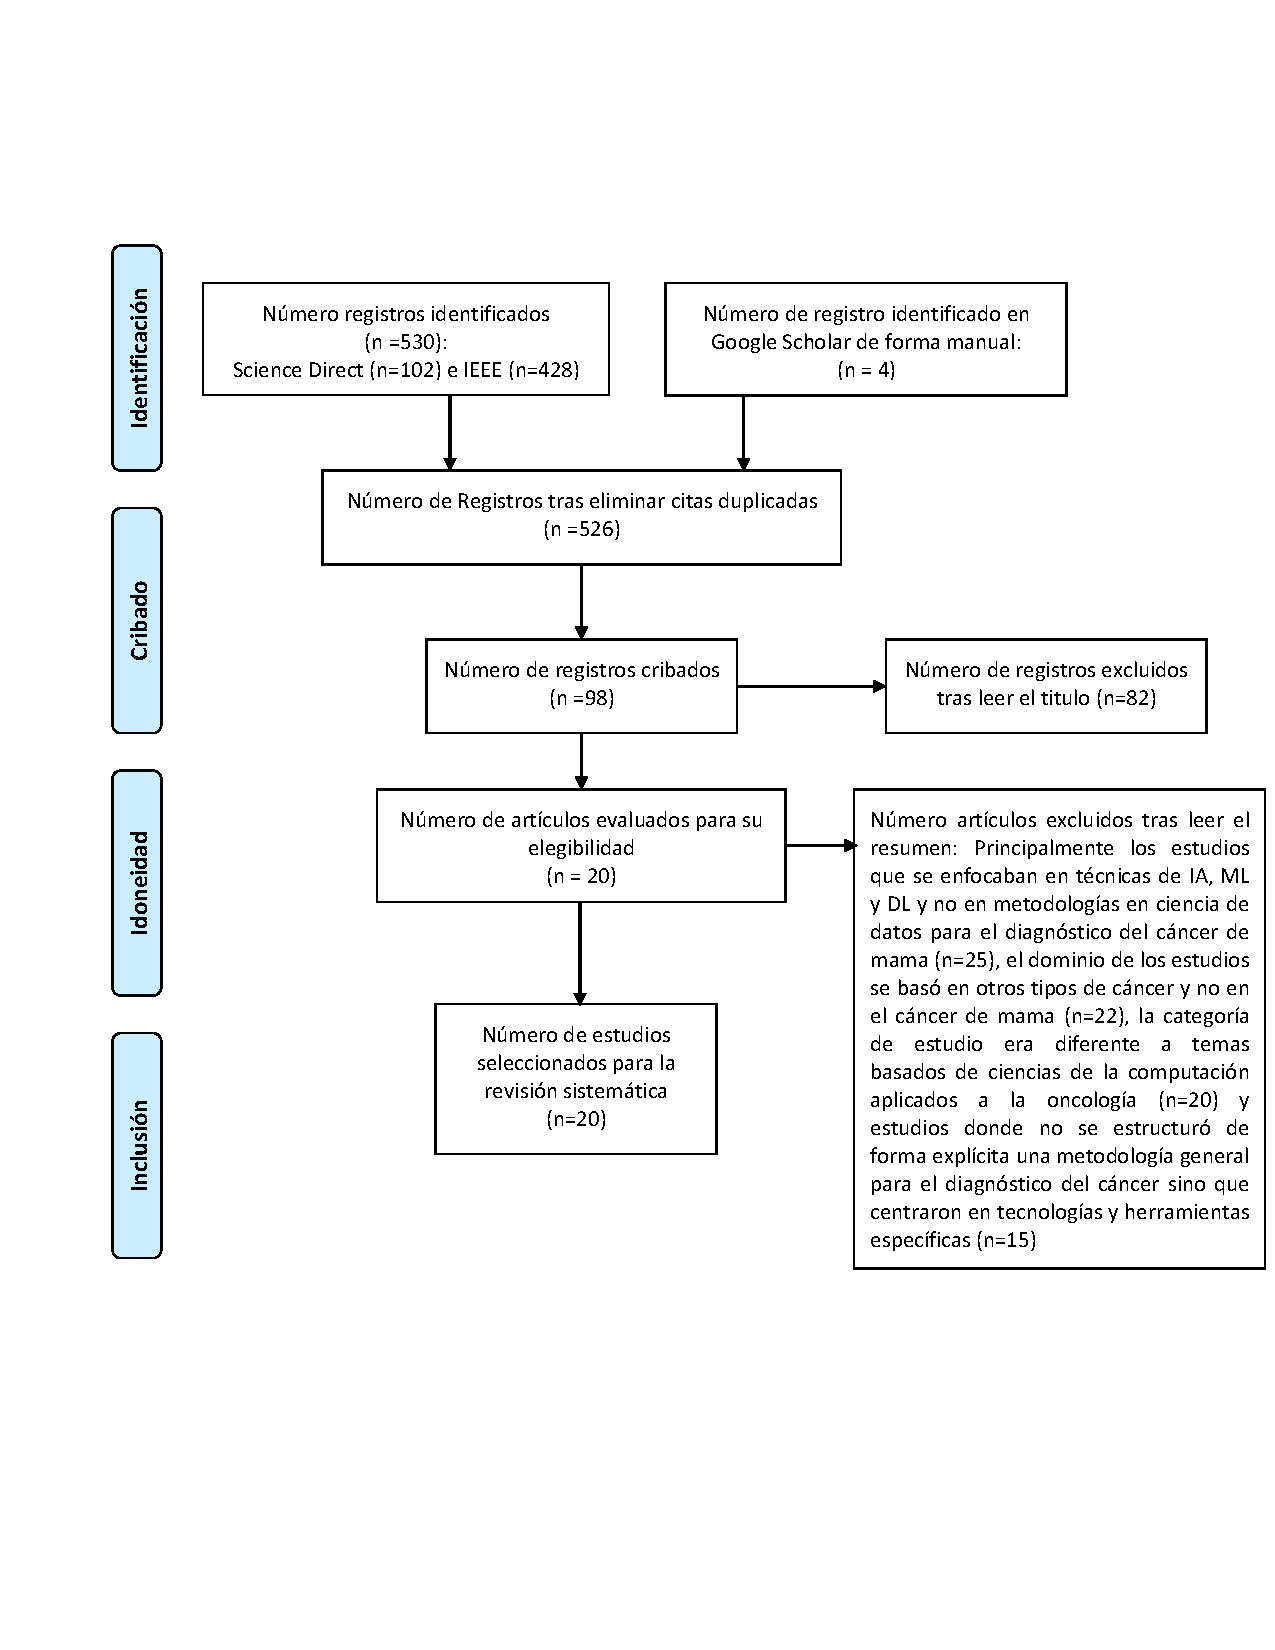
\includegraphics[width=1
	\linewidth]{IMAGENES/PRISMA_DIAGRAM}
	\caption{Diagrama de flujo PRISMA en cuatro niveles }
	\label{Diagrama_Prisma}
\end{figure}

\subsection{Búsqueda inicial}
Las primeras búsquedas se realizaron en abril de 2021 combinando los términos \textit{data science, breast cancer, deep learning, machine Learning, artificial intelligence, cancer Biopsy ,Core needle biopsy, Fine needle aspiration} en las bases de datos de IEEE Access, Nature Reviews Cancer, Elsevier y Science Direct. Posteriormente, para generar una búsqueda mas especifica acerca de metodologías en ciencia de datos aplicadas al diagnostico del cáncer de mama se realizó la combinación de estos términos usando los operadores booleanos \textit{AND} y \textit{OR}. Los resultados obtenidos en la búsqueda arrojaron una cantidad excesiva de literatura basada en técnicas de Inteligencia Artificial, Machine Learning y Deep Learning aplicadas al diagnostico de esta enfermedad sin tener una metodología clara en ciencia de datos aplicada a esta área de la salud, por lo cual dichos resultados fueron poco útiles para la revisión. Sin embargo, las consultas realizadas permitieron tener un visión global de la complejidad del tema de investigación y los diferentes enfoques que pueden generarse a nivel de ciencia de la computación si no se limita la temática al rededor de una metodología.

Debido a que los resultados arrojados por Nature Reviews Cancer y The Lancet estaban enfocados en técnicas y no metodologías, lo cual no aportada información relevante al estudio, se decidió su eliminación de la búsqueda sistemática.  

\subsection{Búsqueda sistemática}
La búsqueda sistemática se realizo en febrero del 2022, en IEEE Access y Science Direct, acotando los resultados de publicaciones realizadas en 2014 hasta la actualidad. La combinación de términos que arrojó mejores resultados en ambos buscadores fue la siguiente:
\textit{(methodology AND Data Science) OR (methodology AND diagnose AND cancer) OR (data science AND methodology AND health AND diagnostics) OR (data science AND methodology AND breast AND cancer)}.

Concretamente, se obtuvieron $530$ resultados de los cuales $428$ fueron encontrados en IEEE Access y $102$ en Science Direct. Antes de realizar la selección de artículos, se definieron los siguientes criterios de inclusión y exclusión. 

\begin{itemize}
	
	\item{\textbf{\textit{Criterios de inclusión}}}
	\begin{itemize}
		\item Tratarse de artículos de investigación, revisión sistemática, libros o manuales. 
		\item Que los estudios realizados estén basadas en metodologías en ciencia de datos  y no en técnicas de Inteligencia Artificial, Machine Learning y Deep Learning.
		\item Que la categoría de estudio este bajo la temática de ciencias de la computación aplicado a la oncología.
		\item Que el dominio determinado este enfocado en el diagnostico del cáncer de mama.
		\item Que los articulo de investigación realizados no dependan de tecnologías ni herramientas específicas.
		\item Que se hayan publicado entre 2014 y 2022, ambos inclusive.
		
	\end{itemize}
	
	\item{\textbf{\textit{Criterios de exclusión}}}
	\begin{itemize}
		\item Se excluyen los estudios que se enfoquen en técnicas de Inteligencia Artificial, Machine Learning y Deep Learning y no en metodologías en ciencia de datos. 
		\item Estudios en donde el dominio se base en otros tipos de cáncer y no en el cáncer de mama.
		\item Estudios donde la categoría sea diferente a temas basados de ciencias de la computación aplicados a la oncología. 
		\item Estudios donde no se evidencie de forma explícita una estrategia general para el diagnóstico del cáncer sino se centren en otros temas, tecnologías y herramientas específicas.
	\end{itemize}
	
\end{itemize}

Según estos criterios, y sólo con la lectura del titulo se consideraron adecuados $98$ artículos. Posteriormente, se realizo la lectura del resumen y a partir de esta lectura, se descartaron $82$ artículos, principalmente los estudios que se enfocaban en técnicas de Inteligencia Artificial, Machine Learning y Deep Learning y no en metodologías en ciencia de datos para el diagnóstico del cáncer de mama ($n=25$), el dominio de los estudios se basó en otros tipos de cáncer y no en el cáncer de mama ($n=22$), la categoría de estudio era diferente a temas basados de ciencias de la computación aplicados a la oncología ($n=20$) y estudios donde no se estructuró de forma explícita una metodología general para el diagnóstico del cáncer sino que centraron en tecnologías y herramientas específicas ($n=15$). Finalmente, $16$ artículos encontrados en IEEE Access y Science Direct cumplieron con los criterios de inclusión y se seleccionaron para llevar a cabo la revisión sistemática. 

\subsection{Búsqueda Manual}
Al realizar una lectura detallada de las $16$ investigaciones encontradas en la búsqueda sistemática, basándonos en sus referencias para comprobar si existía información adicional relacionada con el tema de estudio, se empleo Google Scholar con los términos de búsqueda descritos anteriormente y como resultado se incluyeron $3$ capítulos de libros de ciencias de la computación que abarcaban diferentes metodologías en ciencia de datos y $1$ articulo de investigación encontrado en la revista IJSR\footnote{International Journal of Science and Research } que contenía información relevante para la investigación. 

En definitiva, $20$ investigaciones entre artículos y capítulos de libros publicados entre 2014 y 2022 fueron seleccionados para realizar la revisión sistemática de la aplicación de la ciencia de datos en metodologías para el diagnóstico del cáncer de mama (Figura \ref{Diagrama_Prisma}).
%\chapter{Resultados}
%\section{Discusión}
Según los resultados obtenidos, se infiere que en la información revisada no existe una metodología en ciencia de datos definida para el diagnóstico del cáncer de mama. En efecto, la mayoría de la literatura científica apunta directamente al uso de técnicas de ML y DL para el diagnóstico o pronostico del cáncer de mama exponiendo el nivel de precisión, cantidad de falsos positivos, gasto computacional y modelos algorítmicos utilizados para determinar el posible padecimiento de esta enfermedad. Y aunque estas investigaciones, brindan información valiosa para mejorar la precisión, sensibilidad y especificidad de las técnicas de ML y DL en el diagnóstico del cáncer, carecen de una metodología clara en donde la idea principal gire entorno de la comprensión del dominio y la toma de decisiones por parte de los oncólogos. En particular, la mayoría de investigaciones llegan a resultados en términos de precisión y exactitud, pero no profundizan en el valor real que el especialista en oncología atribuye a los datos para tomar una decisión y el impacto que dicha decisión tiene en la usabilidad del modelo generado, a sabiendas que el experto a través de su perspicacia medica es quien finalmente evalúa si los resultados obtenidos por los algoritmos son veraces y permiten diagnosticar el cáncer de forma ágil, generando un valor agregado que cumpla con los objetivos de las ciencias de la salud. Por consiguiente, aunque la comunidad de investigación en ciencia de datos este en crecimiento constante, esté explorando nuevos dominios, creando nuevos roles especializados y este realizando un gran esfuerzo de investigación para desarrollar análisis avanzados, mejorar modelos de datos y generar nuevos algoritmos apoyados de los campos de las matemáticas, la estadística y la informática, estas habilidades no son suficientes para la aplicación de la ciencia de datos en proyectos reales \citep{Martinez2021}, puesto que la mayoría de proyectos basados en datos presentan problemas organizativos y socio-técnicos, tales como: una falta de visión y claridad en los objetivos, un énfasis sesgado en cuestiones técnicas y ambigüedad de los roles. Dicho lo anterior, aunque las metodologías seleccionadas en la revisión sistemática no giren en torno al cáncer, proponen etapas que abarcan aspectos relevantes en la organización, a nivel de planteamiento y ejecución de un proyecto en ciencia de datos que tiene como eje el dominio basado en la prevención, el diagnostico y el tratamiento del cáncer de mama. Cabe resaltar que las metodologías CRISP-DM y KDD fueron seleccionadas debido a que comprenden todas las fases básicas que debe cumplir cualquier proyecto que tenga en su contexto el análisis de datos, ademas de que son bastante utilizadas por una cantidad considerable de investigadores, sin embargo aunque sean las metodologías más utilizadas, carecen de lineamientos que profundicen en la organización de los equipos de trabajo para llevar a cabo procesos de gestión que se alienen con el software y las metodologías de desarrollo ágiles. Ademas, autores como \citep{Martinez2021} sugieren que para ofrecer una solución integral para la ejecución exitosa de una metodología en ciencia de datos se deben cubrir estrictamente tres áreas: gestión de proyectos, gestión de equipos y gestión de datos e información. 
Por consiguiente, tras el esfuerzo por integrar los resultados analizados en este trabajo, parece bastante plausible afirmar que no existe una metodología puntual en ciencia de datos que se enfoque en el diagnóstico del cáncer de mama, sin embargo, diversos autores proponen metodologías que permiten la aplicación de esta ciencia en el dominio de las ciencias de la salud, teniendo como eje principal la comprensión de aspectos como: la comunicación constante con los interesados, el uso del enfoque ágil, la definición de roles y funciones, el valor agregado de los datos, la retroalimentación continua y la aceptación del experto en oncología para la posterior toma de decisiones que ayude a reducir de manera eficaz la morbilidad causada por esta enfermedad.


% PASA uses footnotes, not endnotes. \endnote in this template will behave like \footnote; and \printendnotes will not output anything.
% \printendnotes
\bibliographystyle{unsrt}
%\bibliographystyle{apalike}
\bibliography{REFERENCIAS/articulos}
%\appendix
%\input{example-appendices}

\end{document}
